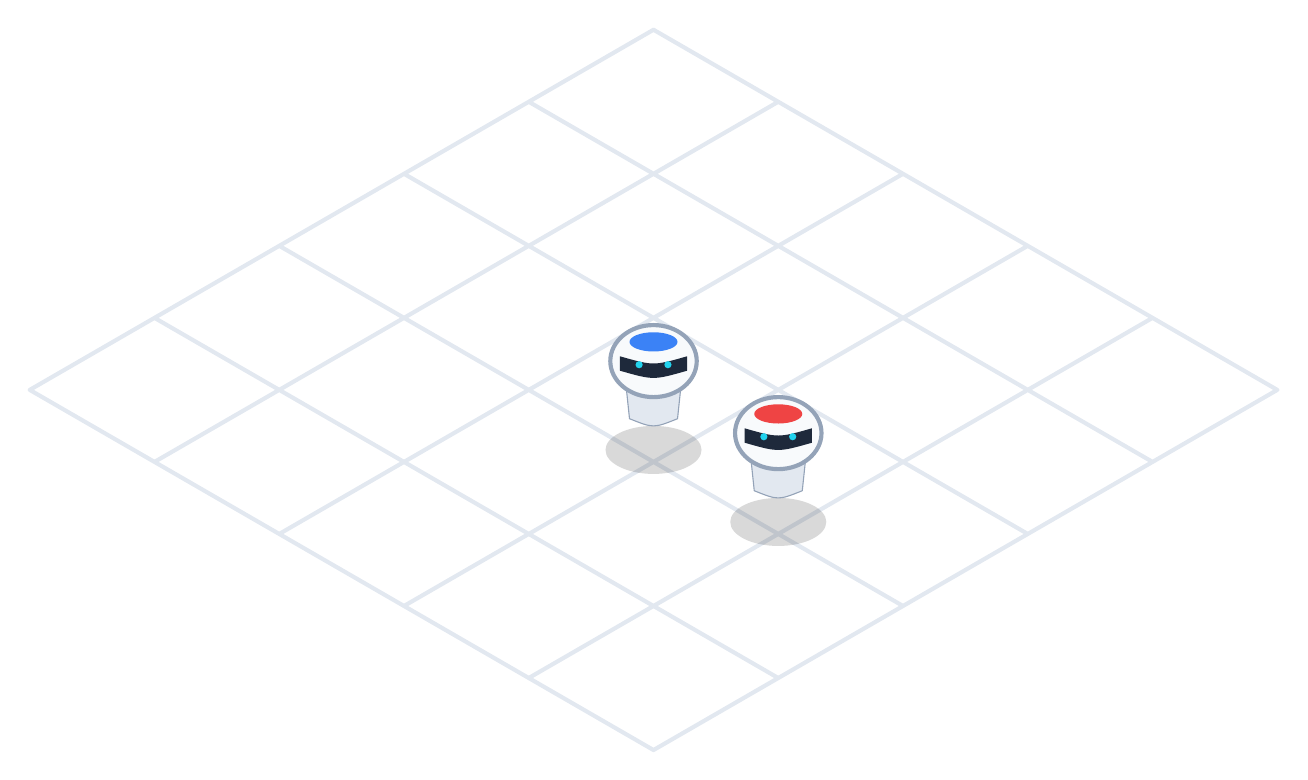
\begin{tikzpicture}[x=0.025cm,y=-0.025cm,line cap=round,line join=round]
\definecolor{gridline}{HTML}{E2E8F0}
\definecolor{robotedge}{HTML}{94A3B8}
\definecolor{robotbody}{HTML}{F8FAFC}
\definecolor{robotbase}{HTML}{E2E8F0}
\definecolor{robotvisor}{HTML}{1E293B}
\definecolor{roboteye}{HTML}{22D3EE}
\definecolor{bluebot}{HTML}{3B82F6}
\definecolor{redbot}{HTML}{EF4444}

\begin{scope}[shift={(0,-28)},scale=1.22]
  % Adjusted grid: Removed one row and one column
  \draw[gridline,line width=1.5]
    % Diagonal lines (NW to SE) - One fewer line
    (0,0) -- (-259.8,150)
    (51.96,30) -- (-207.84,180)
    (103.92,60) -- (-155.88,210)
    (155.88,90) -- (-103.92,240)
    (207.84,120) -- (-51.96,270)
    (259.8,150) -- (0,300)

    % Diagonal lines (NE to SW) - One fewer line
    (0,0) -- (259.8,150)
    (-51.96,30) -- (207.84,180)
    (-103.92,60) -- (155.88,210)
    (-155.88,90) -- (103.92,240)
    (-207.84,120) -- (51.96,270)
    (-259.8,150) -- (0,300);

  \foreach \x/\y/\capcolor in {0/150/bluebot,51.96/180/redbot} {
    \begin{scope}[shift={(\x,\y)}]
      \fill[black,opacity=0.15] (0,25) ellipse [x radius=20,y radius=10];
      \begin{scope}[shift={(0,-12)}]
        \filldraw[fill=robotbase,draw=robotedge]
          (-12,5) -- (12,5) -- (10,24)
          .. controls (0,28) .. (-10,24) -- cycle;
        \filldraw[fill=robotbody,draw=robotedge,line width=1.5]
          (0,0) ellipse [x radius=18,y radius=15];
        \fill[robotvisor]
          (-14,-2) .. controls (0,2) .. (14,-2)
          -- (14,4) .. controls (0,8) .. (-14,4) -- cycle;
        \fill[roboteye] (-6,1.5) circle [radius=1.5];
        \fill[roboteye] (6,1.5) circle [radius=1.5];
        \fill[\capcolor] (0,-8) ellipse [x radius=10,y radius=4];
      \end{scope}
    \end{scope}
  }
\end{scope}
\end{tikzpicture}
